\documentclass[tikz,border=6pt]{standalone}
\usepackage{amsmath}
\usepackage{xcolor}
\usetikzlibrary{arrows.meta,positioning,calc}

\definecolor{blockblue}{HTML}{4A90D9}
\definecolor{sumgreen}{HTML}{5CB85C}
\definecolor{taporange}{HTML}{F0AD4E}
\definecolor{signalgray}{HTML}{333333}

\tikzset{
  block/.style={rectangle, draw=blockblue, fill=none, minimum width=1.55cm, minimum height=0.70cm, line width=1.2pt, align=center, font=\footnotesize\bfseries},
  sum/.style={circle, draw=sumgreen, fill=none, minimum size=0.45cm, inner sep=0pt, line width=1.2pt,
    path picture={
      \draw[sumgreen,line width=1.0pt] ($(path picture bounding box.center)+(-0.12,-0.12)$) -- ($(path picture bounding box.center)+(0.12,0.12)$);
      \draw[sumgreen,line width=1.0pt] ($(path picture bounding box.center)+(-0.12,0.12)$) -- ($(path picture bounding box.center)+(0.12,-0.12)$);
    }},
  tap/.style={circle, draw=taporange, fill=none, minimum size=4.5pt, inner sep=0pt, line width=1.2pt},
  signal/.style={-{Stealth[length=2.2mm,width=1.6mm]}, draw=signalgray, line width=1.2pt},
  line/.style={draw=signalgray, line width=1.2pt},
  neg sign/.style={font=\scriptsize\bfseries, fill=white, inner sep=1pt}
}

\begin{document}
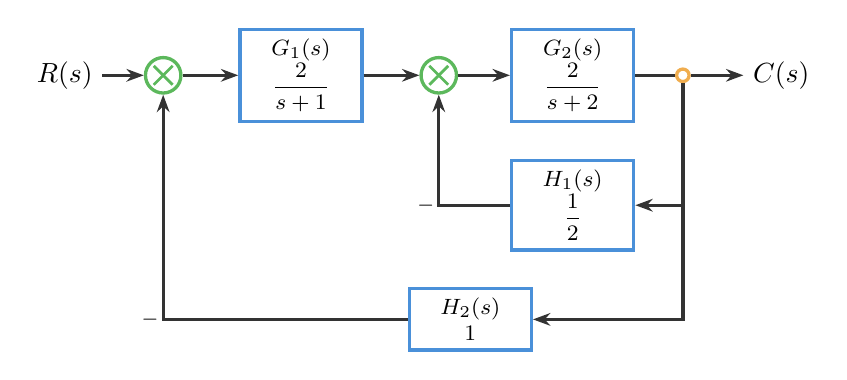
\begin{tikzpicture}[auto, node distance=1.35cm]
  \node (R) at (0,0) {$R(s)$};
  \node[sum] (sum1) at (1.25,0) {};
  \node[block] (G1) at (3.0,0) {$G_1(s)$\\$\dfrac{2}{s+1}$};
  \node[sum] (sum2) at (4.75,0) {};
  \node[block] (G2) at (6.45,0) {$G_2(s)$\\$\dfrac{2}{s+2}$};
  \node[tap] (tapout) at (7.85,0) {};
  \node (C) at (9.10,0) {$C(s)$};

  \draw[signal] (R) -- (sum1);
  \draw[signal] (sum1) -- (G1);
  \draw[signal] (G1) -- (sum2);
  \draw[signal] (sum2) -- (G2);
  \draw[signal] (G2) -- (tapout) -- (C);

  \node[block] (H1) at (6.45,-1.65) {$H_1(s)$\\$\dfrac{1}{2}$};
  \draw[line] (tapout) -- ++(0,-0.55);
  \draw[signal] ($(tapout)+(0,-0.55)$) |- (H1);
  \draw[signal] (H1) -| node[neg sign, left] {$-$} (sum2.south);

  \node[block] (H2) at (5.15,-3.10) {$H_2(s)$\\$1$};
  \draw[line] (tapout) -- ++(0,-2.15);
  \draw[signal] ($(tapout)+(0,-2.15)$) |- (H2);
  \draw[signal] (H2) -| node[neg sign, left] {$-$} (sum1.south);
\end{tikzpicture}
\end{document}
